\documentclass[10pt]{article}
\usepackage[polish]{babel}
\usepackage[utf8]{inputenc}
\usepackage[T1]{fontenc}
\usepackage{graphicx}
\usepackage[export]{adjustbox}
\graphicspath{ {./images/} }
\usepackage{amsmath}
\usepackage{amsfonts}
\usepackage{amssymb}
\usepackage[version=4]{mhchem}
\usepackage{stmaryrd}

\title{Zestaw 14 }

\author{}
\date{}


\newcommand\Varangle{\mathop{{<\!\!\!\!\!\text{\small)}}\:}\nolimits}

\begin{document}
\maketitle
\begin{center}

\includegraphics[max width=\textwidth]{2024_11_21_a3b3d3b4a87def3715fbg-1(1)}
\end{center}

\begin{enumerate}
  \item Dany jest prostokąt \(A B C D\). Budujemy na jego bokach \(A B\) i \(B C\), po jego wewnętrznej stronie, trójkąty równoboczne \(A B E\) i \(B C F\). Udowodnij, że trójkąt \(D E F\) jest równoboczny.\\
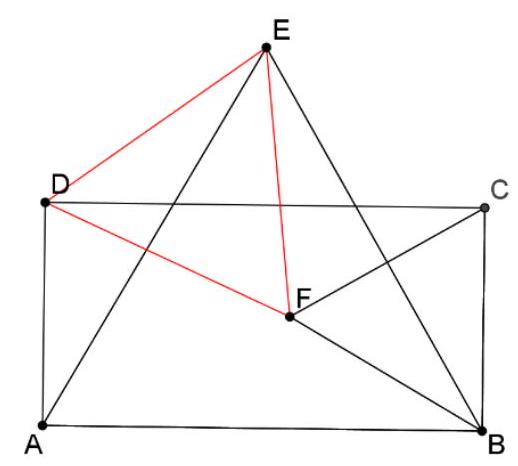
\includegraphics[max width=\textwidth, center]{2024_11_21_a3b3d3b4a87def3715fbg-1}
  \item Punkty \(P\) i \(Q\) leżą odpowiednio na bokach \(B C\) i \(C D\) kwadratu \(A B C D\), przy czym \(P B+D Q=P Q\). Udowodnij, że \(\Varangle Q A P=45^{\circ}\).
  \item Dany jest czworokąt wypukły \(A B C D\), w którym \(\Varangle D A B=\Varangle A B C\). Symetralne odcinków \(A D\) i \(B C\) przecinają się w punkcie \(M\) leżącym na odcinku \(A B\). Udowodnić, że \(A C=B D\).\\
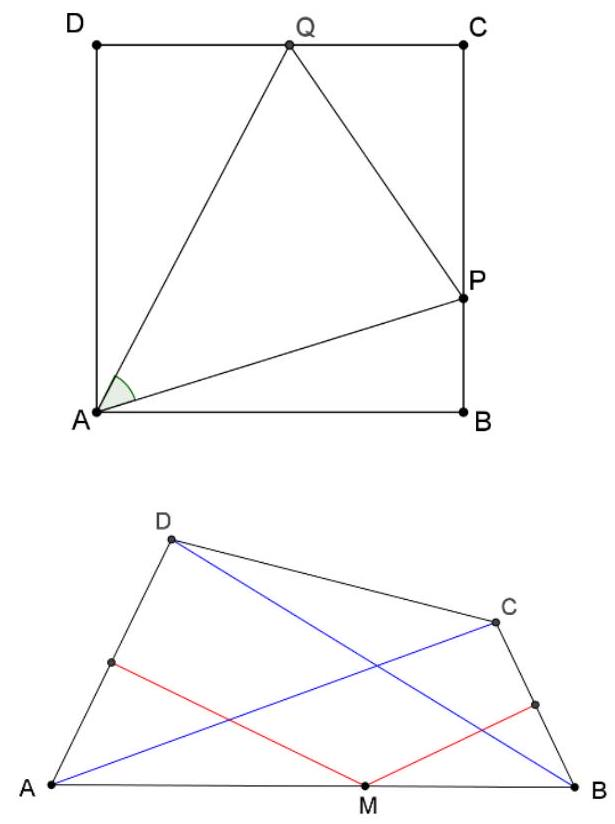
\includegraphics[max width=\textwidth, center]{2024_11_21_a3b3d3b4a87def3715fbg-1(2)}
\end{enumerate}

\end{document}